\documentclass{article}
\usepackage[utf8]{inputenc}
\usepackage{amsthm,amsmath,bm,bbm}
\usepackage{amssymb,mathtools}
\usepackage[dvipsnames]{xcolor}
\usepackage[colorlinks=true, allcolors=violet]{hyperref}
\usepackage{tikz}
\usetikzlibrary{shapes,shadows,arrows,positioning,arrows.meta,decorations.pathreplacing,decorations.pathmorphing,decorations.shapes}
\usepackage[colorinlistoftodos,textsize=scriptsize,textwidth=.8in,color=blue!20]{todonotes}

\begin{document}

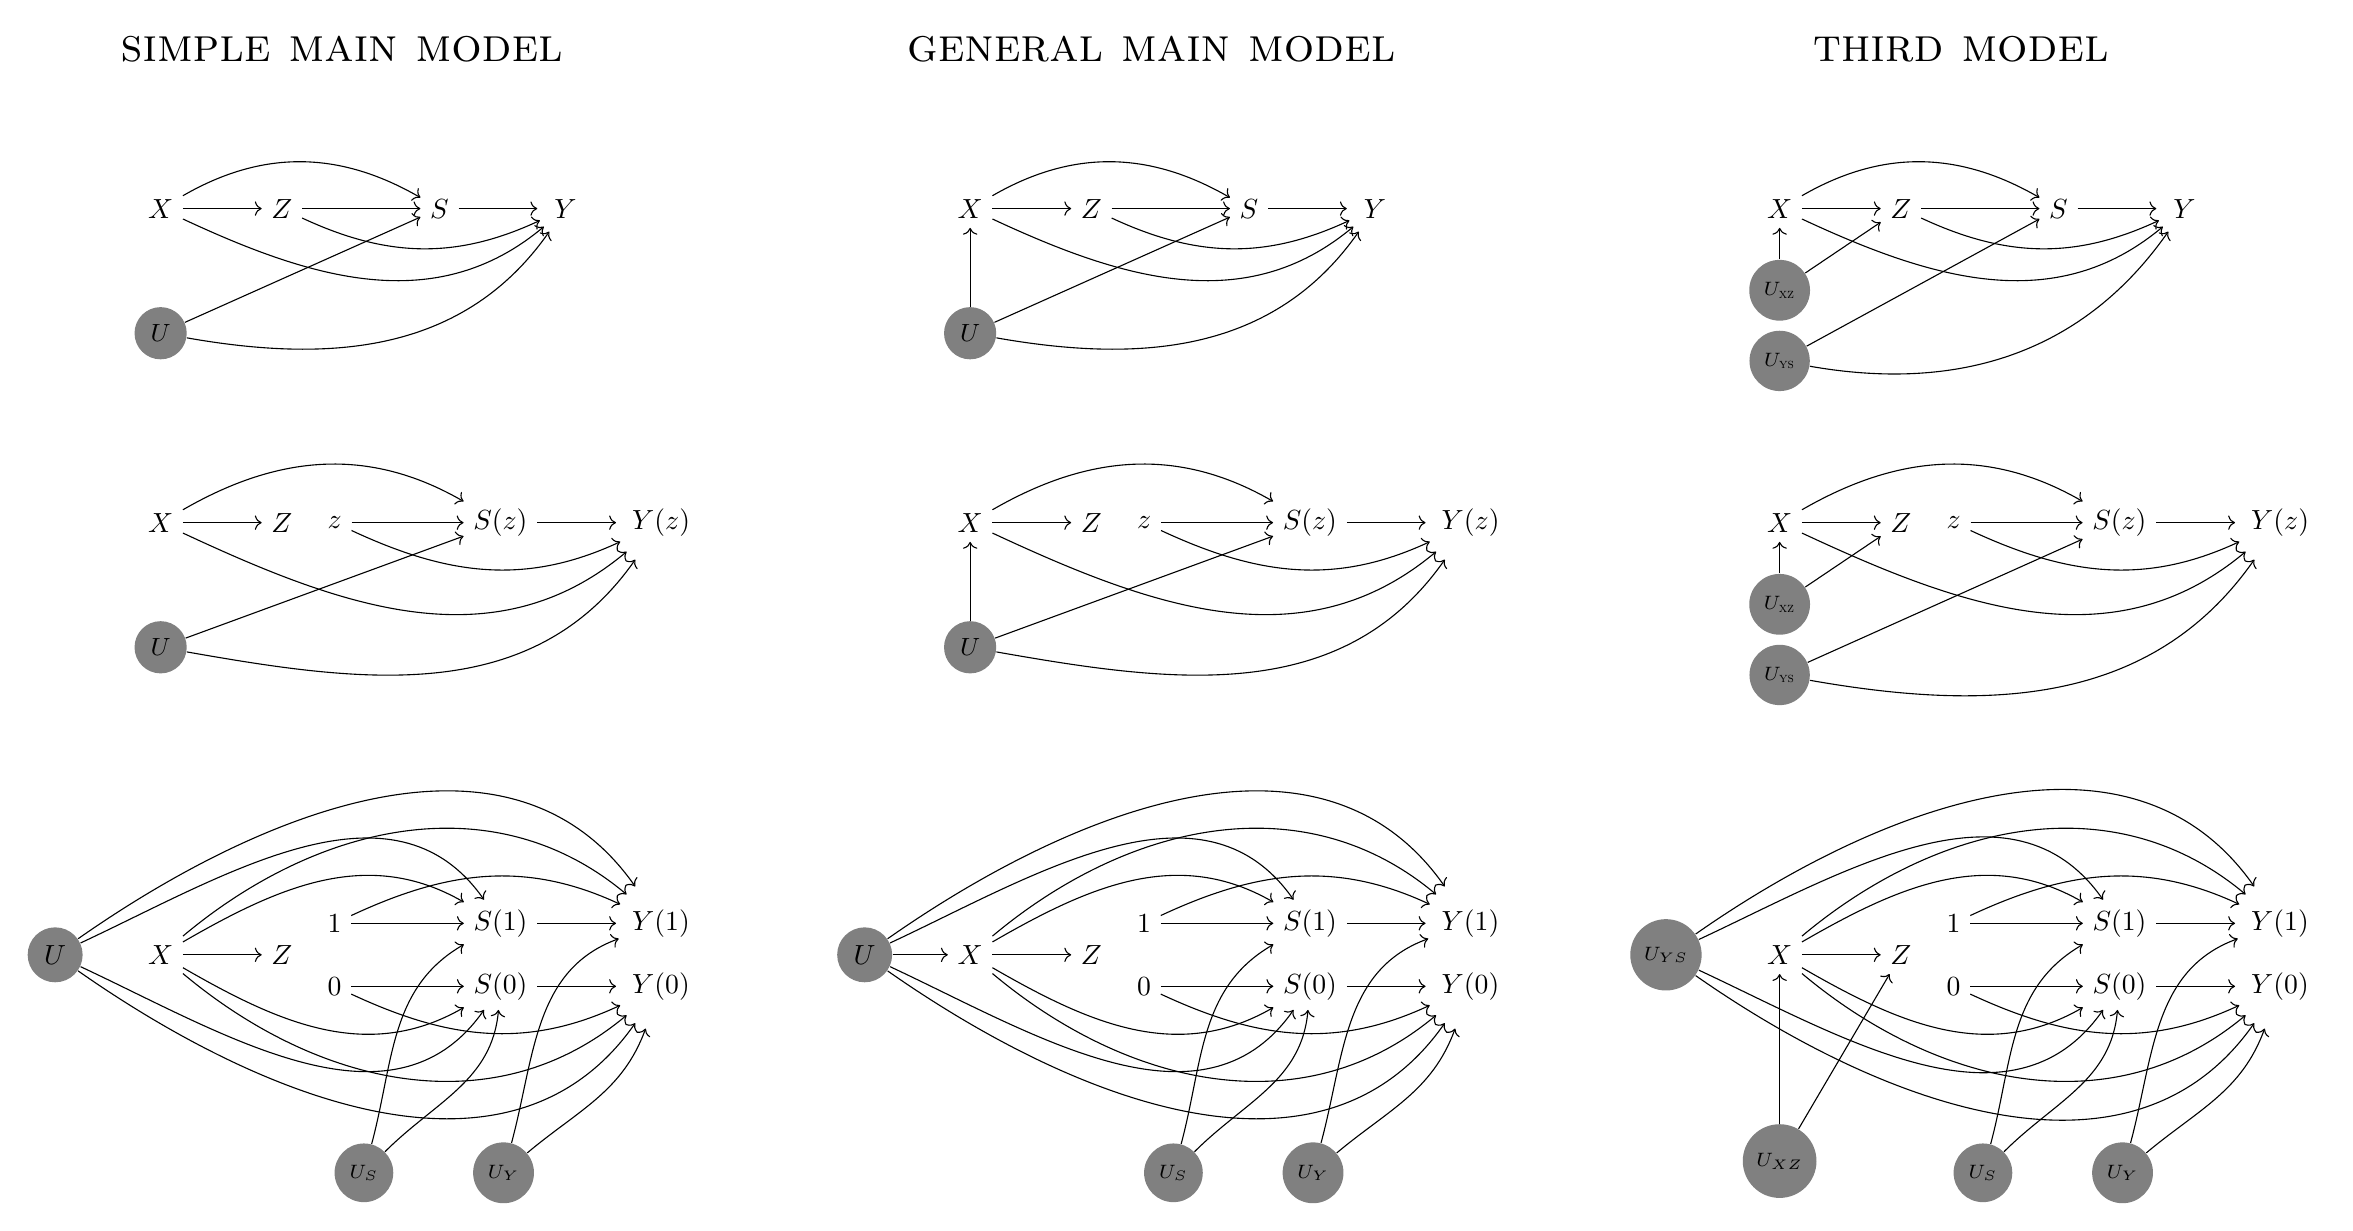
\begin{tikzpicture}[
    v/.style={rectangle, minimum width=1mm, minimum size=1mm, text centered},
    c/.style={circle, fill = gray!20},
    s/.style={diamond, fill = gray},
    u/.style={circle, fill = gray},
    o/.style={circle}]

        % D %%%%%%%%%%%%%%%%%%%%%%%%%%%%%%%%
        \node[v] (X) {${X}$};
        \node[v] (Z) [right=of X] {${Z}$};
        \node[o] (Y) [right=of X, xshift=35mm] {$Y$};
        \node[v] (S) [left=of Y] {$S$};
        \node[u] (U) [below=of X] {\small $U$};
        
        \draw[->] (X) -- (Z);
        
        \draw[->] (X) to[out=30,in=150] (S);
        \draw[->] (Z) -- (S);
        \draw[->] (U) -- (S);
        
        \draw[->] (X) to[out=-25,in=220] (Y);
        \draw[->] (Z) to[out=-25,in=-155] (Y);
        \draw[->] (S) -- (Y);
        \draw[->] (U) to[out=-10, in=235] (Y);

        \node[v] [above=of X, xshift=23mm, yshift=5mm] {\LARGE\textsc{simple main model}};

        
        \node[v] (X2) [below=of X, yshift=-25mm] {${X}$};
        \node[v] (Z2) [right=of X2] {${Z}$};
        \node[v] (z2) [right=of Z2, xshift=-8mm] {$z$};
        \node[o] (Y2) [right=of X2, xshift=45mm] {$Y(z)$};
        \node[v] (S2) [left=of Y2] {$S(z)$};
        \node[u] (U2) [below=of X2] {\small $U$};
        
        \draw[->] (X2) -- (Z2);
        
        \draw[->] (X2) to[out=30,in=150] (S2);
        \draw[->] (z2) -- (S2);
        \draw[->] (U2) -- (S2);
        
        \draw[->] (X2) to[out=-25,in=220] (Y2);
        \draw[->] (z2) to[out=-25,in=-155] (Y2);
        \draw[->] (S2) -- (Y2);
        \draw[->] (U2) to[out=-10, in=235] (Y2);



        \node[v] (X) [below=of X2, yshift=-40mm] {${X}$};
        \node[v] (Z) [right=of X] {${Z}$};
        \node[u] (U) [left=of X, xshift=3mm] {$U$};
        \node[v] (z1) [right=of Z, xshift=-8mm, yshift=4mm] {$1$};
        \node[o] (Y1) [right=of X, xshift=45mm, yshift=4mm] {$Y(1)$};
        \node[v] (S1) [left=of Y1] {$S(1)$};
        \node[v] (z0) [right=of Z, xshift=-8mm, yshift=-4mm] {$0$};
        \node[o] (Y0) [right=of X, xshift=45mm, yshift=-4mm] {$Y(0)$};
        \node[v] (S0) [left=of Y0] {$S(0)$};
        \node[u] (Us) [below left=of S0, yshift=-8mm] {\scriptsize$U_{\scriptscriptstyle S}$};
        \node[u] (Uy) [right=of Us] {\scriptsize$U_{\scriptscriptstyle Y}$};
        
        \draw[->] (X) -- (Z);
        
        \draw[->] (X) to[out=30,in=150] (S1);
        \draw[->] (z1) -- (S1);
        \draw[->] (U) to [out=25, in=125] (S1);
        
        \draw[->] (X) to[out=-30,in=-150] (S0);
        \draw[->] (z0) -- (S0);
        \draw[->] (U) to [out=-25, in=-125] (S0);
        
        \draw[->] (X) to[out=40,in=140] (Y1);
        \draw[->] (z1) to[out=25,in=155] (Y1);
        \draw[->] (S1) -- (Y1);
        \draw[->] (U) to[out=35, in=125] (Y1);

        \draw[->] (X) to[out=-40,in=220] (Y0);
        \draw[->] (z0) to[out=-25,in=-155] (Y0);
        \draw[->] (S0) -- (Y0);
        \draw[->] (U) to[out=-35, in=-125] (Y0);

        
        \draw[->] (Us) to [out=75, in=-150] (S1);
        \draw[->] (Us) to [out=45, in=-95] (S0);
        \draw[->] (Uy) to [out=75, in=-160] (Y1);
        \draw[->] (Uy) to [out=40, in=-110] (Y0);
        


        % D %%%%%%%%%%%%%%%%%%%%%%%%%%%%%%%%
        \node[v] (X) [right=of Y, xshift=35mm] {${X}$};
        \node[v] (Z) [right=of X] {${Z}$};
        \node[o] (Y) [right=of X, xshift=35mm] {$Y$};
        \node[v] (S) [left=of Y] {$S$};
        \node[u] (U) [below=of X] {\small $U$};
        
        \draw[->] (U) -- (X);
        
        \draw[->] (X) -- (Z);
        
        \draw[->] (X) to[out=30,in=150] (S);
        \draw[->] (Z) -- (S);
        \draw[->] (U) -- (S);
        
        \draw[->] (X) to[out=-25,in=220] (Y);
        \draw[->] (Z) to[out=-25,in=-155] (Y);
        \draw[->] (S) -- (Y);
        \draw[->] (U) to[out=-10, in=235] (Y);

        \node[v] [above=of X, xshift=23mm, yshift=5mm] {\LARGE\textsc{general main model}};

        
        \node[v] (X2) [below=of X, yshift=-25mm] {${X}$};
        \node[v] (Z2) [right=of X2] {${Z}$};
        \node[v] (z2) [right=of Z2, xshift=-8mm] {$z$};
        \node[o] (Y2) [right=of X2, xshift=45mm] {$Y(z)$};
        \node[v] (S2) [left=of Y2] {$S(z)$};
        \node[u] (U2) [below=of X2] {\small $U$};
        
        \draw[->] (U2) -- (X2);
        
        \draw[->] (X2) -- (Z2);
        
        \draw[->] (X2) to[out=30,in=150] (S2);
        \draw[->] (z2) -- (S2);
        \draw[->] (U2) -- (S2);
        
        \draw[->] (X2) to[out=-25,in=220] (Y2);
        \draw[->] (z2) to[out=-25,in=-155] (Y2);
        \draw[->] (S2) -- (Y2);
        \draw[->] (U2) to[out=-10, in=235] (Y2);


        \node[v] (X) [below=of X2, yshift=-40mm] {${X}$};
        \node[v] (Z) [right=of X] {${Z}$};
        \node[u] (U) [left=of X, xshift=3mm] {$U$};
        \node[v] (z1) [right=of Z, xshift=-8mm, yshift=4mm] {$1$};
        \node[o] (Y1) [right=of X, xshift=45mm, yshift=4mm] {$Y(1)$};
        \node[v] (S1) [left=of Y1] {$S(1)$};
        \node[v] (z0) [right=of Z, xshift=-8mm, yshift=-4mm] {$0$};
        \node[o] (Y0) [right=of X, xshift=45mm, yshift=-4mm] {$Y(0)$};
        \node[v] (S0) [left=of Y0] {$S(0)$};
        \node[u] (Us) [below left=of S0, yshift=-8mm] {\scriptsize$U_{\scriptscriptstyle S}$};
        \node[u] (Uy) [right=of Us] {\scriptsize$U_{\scriptscriptstyle Y}$};
        
        \draw[->] (U) -- (X);
        
        \draw[->] (X) -- (Z);
        
        \draw[->] (X) to[out=30,in=150] (S1);
        \draw[->] (z1) -- (S1);
        \draw[->] (U) to [out=25, in=125] (S1);
        
        \draw[->] (X) to[out=-30,in=-150] (S0);
        \draw[->] (z0) -- (S0);
        \draw[->] (U) to [out=-25, in=-125] (S0);
        
        \draw[->] (X) to[out=40,in=140] (Y1);
        \draw[->] (z1) to[out=25,in=155] (Y1);
        \draw[->] (S1) -- (Y1);
        \draw[->] (U) to[out=35, in=125] (Y1);

        \draw[->] (X) to[out=-40,in=220] (Y0);
        \draw[->] (z0) to[out=-25,in=-155] (Y0);
        \draw[->] (S0) -- (Y0);
        \draw[->] (U) to[out=-35, in=-125] (Y0);

        
        \draw[->] (Us) to [out=75, in=-150] (S1);
        \draw[->] (Us) to [out=45, in=-95] (S0);
        \draw[->] (Uy) to [out=75, in=-160] (Y1);
        \draw[->] (Uy) to [out=40, in=-110] (Y0);


        


        % D %%%%%%%%%%%%%%%%%%%%%%%%%%%%%%%%
        \node[v] (X) [right=of Y, xshift=35mm] {${X}$};
        \node[v] (Z) [right=of X] {${Z}$};
        \node[o] (Y) [right=of X, xshift=35mm] {$Y$};
        \node[v] (S) [left=of Y] {$S$};
        \node[u] (U) [below=of X, yshift=-3mm] {\scriptsize $U_\textsc{ys}$};
        \node[u] (Uz) [below=of X, yshift=6mm] {\scriptsize $U_\textsc{xz}$};
        
        \draw[->] (Uz) -- (X);
        
        \draw[->] (X) -- (Z);
        \draw[->] (Uz) -- (Z);
        
        \draw[->] (X) to[out=30,in=150] (S);
        \draw[->] (Z) -- (S);
        \draw[->] (U) -- (S);
        
        \draw[->] (X) to[out=-25,in=220] (Y);
        \draw[->] (Z) to[out=-25,in=-155] (Y);
        \draw[->] (S) -- (Y);
        \draw[->] (U) to[out=-10, in=235] (Y);

        \node[v] [above=of X, xshift=23mm, yshift=5mm] {\LARGE\textsc{third model}};

        
        \node[v] (X2) [below=of X, yshift=-25mm] {${X}$};
        \node[v] (Z2) [right=of X2] {${Z}$};
        \node[v] (z2) [right=of Z2, xshift=-8mm] {$z$};
        \node[o] (Y2) [right=of X2, xshift=45mm] {$Y(z)$};
        \node[v] (S2) [left=of Y2] {$S(z)$};
        \node[u] (U2) [below=of X2, yshift=-3mm] {\scriptsize $U_\textsc{ys}$};
        \node[u] (Uz2) [below=of X2, yshift=6mm] {\scriptsize $U_\textsc{xz}$};
        
        \draw[->] (Uz2) -- (X2);
        
        \draw[->] (X2) -- (Z2);
        \draw[->] (Uz2) -- (Z2);
        
        \draw[->] (X2) to[out=30,in=150] (S2);
        \draw[->] (z2) -- (S2);
        \draw[->] (U2) -- (S2);
        
        \draw[->] (X2) to[out=-25,in=220] (Y2);
        \draw[->] (z2) to[out=-25,in=-155] (Y2);
        \draw[->] (S2) -- (Y2);
        \draw[->] (U2) to[out=-10, in=235] (Y2);


        \node[v] (X) [below=of X2, yshift=-40mm] {${X}$};
        \node[v] (Z) [right=of X] {${Z}$};
        \node[u] (U) [left=of X, xshift=3mm] {\scriptsize$U_{\scriptscriptstyle YS}$};
        \node[v] (z1) [right=of Z, xshift=-8mm, yshift=4mm] {$1$};
        \node[o] (Y1) [right=of X, xshift=45mm, yshift=4mm] {$Y(1)$};
        \node[v] (S1) [left=of Y1] {$S(1)$};
        \node[v] (z0) [right=of Z, xshift=-8mm, yshift=-4mm] {$0$};
        \node[o] (Y0) [right=of X, xshift=45mm, yshift=-4mm] {$Y(0)$};
        \node[v] (S0) [left=of Y0] {$S(0)$};
        \node[u] (Us) [below left=of S0, yshift=-8mm] {\scriptsize$U_{\scriptscriptstyle S}$};
        \node[u] (Uy) [right=of Us] {\scriptsize$U_{\scriptscriptstyle Y}$};
        \node[u] (Uxz) [below=of X, yshift=-9mm] {\scriptsize$U_{\scriptscriptstyle XZ}$};
        
        \draw[->] (Uxz) -- (X);
        \draw[->] (Uxz) -- (Z);
        
        \draw[->] (X) -- (Z);
        
        \draw[->] (X) to[out=30,in=150] (S1);
        \draw[->] (z1) -- (S1);
        \draw[->] (U) to [out=25, in=125] (S1);
        
        \draw[->] (X) to[out=-30,in=-150] (S0);
        \draw[->] (z0) -- (S0);
        \draw[->] (U) to [out=-25, in=-125] (S0);
        
        \draw[->] (X) to[out=40,in=140] (Y1);
        \draw[->] (z1) to[out=25,in=155] (Y1);
        \draw[->] (S1) -- (Y1);
        \draw[->] (U) to[out=35, in=125] (Y1);

        \draw[->] (X) to[out=-40,in=220] (Y0);
        \draw[->] (z0) to[out=-25,in=-155] (Y0);
        \draw[->] (S0) -- (Y0);
        \draw[->] (U) to[out=-35, in=-125] (Y0);

        
        \draw[->] (Us) to [out=75, in=-150] (S1);
        \draw[->] (Us) to [out=45, in=-95] (S0);
        \draw[->] (Uy) to [out=75, in=-160] (Y1);
        \draw[->] (Uy) to [out=40, in=-110] (Y0);

\end{tikzpicture}

\end{document}